
\section{Discussion}
\label{sec:discussion}

\subsection{Model interpretation}
The replicator-mutator equations are a mathematical model motivated by concepts from the theory of natural selection, namely natural variation, differential reproduction, and mutation.
The most straightforward interpretation is thus a biological one: we can imagine signaling strategies as innate behaviorial tendencies of organisms, steps in the evolutionary process as successive generations, and selection as capturing the reproductive advantage of fitter individuals.
In this interpretation, our proposed model is not an extremely interesting one, since the noise matrix simply corresponds to a restricted form of mutation.

Another possibility is to take the equations as embodying cultural evolution.
In this interpretation, what is subject to the evolutionary forces are not organisms but strategies themselves.
This pressuposes that individuals can adopt strategies from other individuals.
Fitness captures the success of strategies, which in the case of language can be thought of in terms of communicative success.
Differential reproduction represents the tendency of more successful strategies to be more likely adopted by individuals, be it through imitation or some learning procedure within the population.
Under this interpretation, the proposed noise perturbation becomes more interesting.
Messages correspond to the overt data available to individuals, whereas states are interpreted as the more private aspect of the behavior.
Futhermore, similarity-maximization games are especially interesting in situations where the number of states largely exceeds the number of messages available.
When trying to adopt another individual's behavior, it is thus more likely that information about states is both less accessible and less practical to elicit, hence justifying a higher likelihood of mistakes and a more pressing need for a certain degree of generalization%
\footnote{The consequence of perturbing a strategy with a noise matrix based on similarity can be seen as ``spreading'' the effects of the fitness of the behavior for a state to its more similar states, which can also be interpreted as generalization}%
.

Finally, the replicator dynamics are also related to some forms of reinforcement learning (\cite{Borgers1997,Hopkins2005,Beggs2005}), and can thus be interpreted in cognitive terms.


\subsection{Relation with previous accounts}

\paragraph{Quantal response equilibria.}
\citet{FrankeJager2010:Vagueness-Signa} suggested a number of ways in
which information processing limitations of signaling agents could
lead to vague strategies. The model that is most clearly related to
the present approach uses the notion of a quantal response, also known
as a logit response or a soft-max function
\citep[e.g.][]{Luce1959:Individual-Choi,McFadden1976:Quantal-Choice-,McKelveyPalfrey1995:Quantal-Respons,McKelveyPalfrey1998:Quantal-Respons,GoereeHolt2008:Quantal-Respons}. A
quantal response function is a paramterized generalization of the
classic best response function. For example, if $U \mycolon \Acts
\rightarrow \mathds{R}$ is the measure of expected utility over
choices $\Acts$ of an agent, then a best response function would have
the agent choose $\act$ only if $U(\act) = \max_{\act' \in \Acts}
U(a)$. A quantal response function rather assumes that agents would
choose $\act$ with a probability proportional to $\expo(\lambda \cdot
U(\act))$, where $\lambda$ is a rationality parameter. If $\lambda
\rightarrow \infty$ we retrieve the behavior of the best response
choice function, but if it is positive but finite, any choice $\act$
will receive a positive probability of being chosen, but acts with
higher expected utility will be more
likely. \citet{FrankeJager2010:Vagueness-Signa} show that quantal
response equilibria of sim-max games, i.e., pairs of sender and
receiver strategies such that the sender strategy is the quantal
response to the expected utilities under the receiver strategy and
vice versa, show the desired marks of vague
signaling. Figure~\ref{fig:exampleQRE_stratsA} shows an example of a
quantal response equilibrium for a sim-max game, as used in our set-up
with $\toler = 0.5$. Sender and receiver strategies look very much
like what evolves under \rdd with modest values of perceptual
imprecision. 

There is a major conceptual difference in the source of vagueness
between the quantal response approach and our favored approach in
terms of perceptual noise. When we choose a lower level of pragmatic
tolerance, like we used in our simulations, the predictions of the
quantal response approach look
different. Figure~\ref{fig:exampleQRE_stratsB} shows such an example
that clearly shows that, unlike the evolving strategies under \rdd,
sender strategies have vague boundaries also towards the end of the
unit intervals. This is because quantal responses equalize message use
far away from the ``prototypical'' interpretation. That this is
conceptually odd shows even more clearly in a case where the state
space is intuitively unbounded, as for instance for the property
``tall''. If the usual interpretation of a ``tall man'' peaks at
around, say, 195cm then when meeting a giant of $n$ meters speaker
would, according to the quantal response approach, be ever more
inclined to describe the giant as ``short''. This is because, as the
distance from the prototype increases for larger $n$, the expected
utilities of saying ``short'' or ``tall'' will both converge to zero,
and the difference between the two will also converge to zero. Whence
that the quantal response approach would predict that speakers would
grow indifferent between choice of antonyms as $n$ grows, which seems
weird. (Notice that this argument hinges on the choice of utility
function. Still, to the extent that the chosen lower bounded utility
functions are reasonable ---and we think they are very reasonable---,
this is a conceptual oddity.)

The \rdd approach does not have this peculiarity. \dots


\begin{figure}
  \centering
  
  \begin{subfigure}[]{0.45\textwidth}
    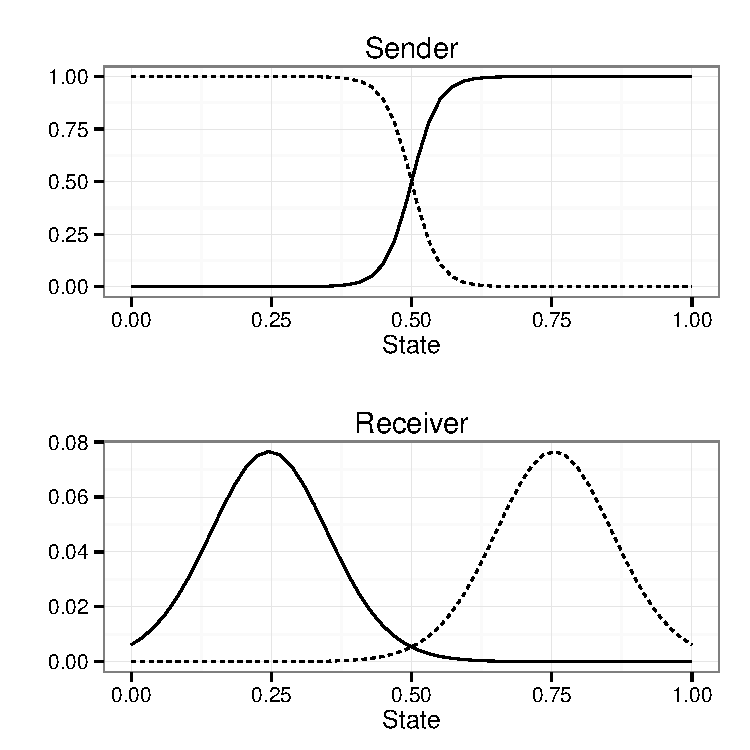
\includegraphics[width=\textwidth]{plots/exampleStratQRE_tolerance05.pdf}
    \caption{$\ns = 90$, $\lambda = 15$, $\toler = 0.5$}
    \label{fig:exampleQRE_stratsA}
  \end{subfigure}
  \hfill
  \begin{subfigure}[]{0.45\textwidth}
    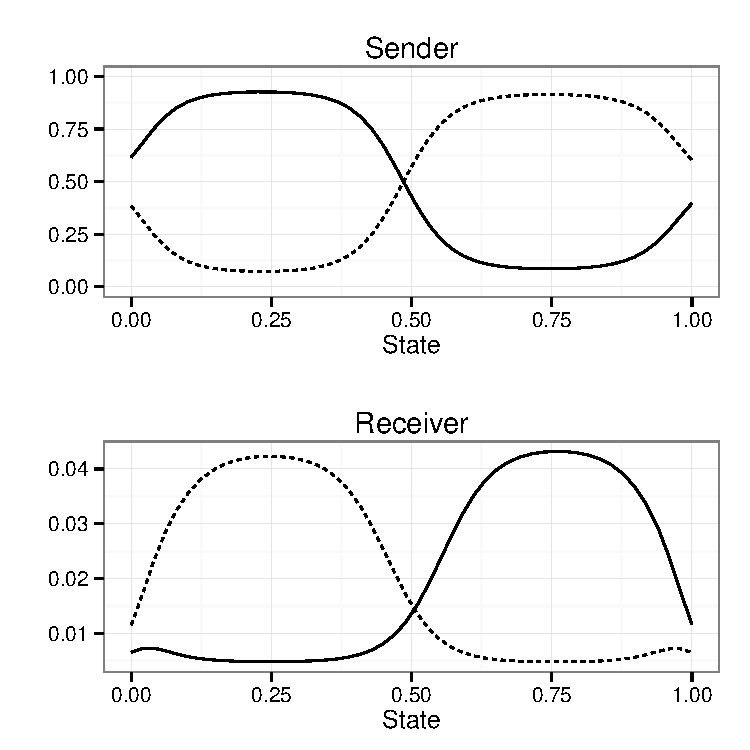
\includegraphics[width=\textwidth]{plots/exampleStratQRE_tolerance005.pdf}
    \caption{$\ns = 90$, $\lambda = 15$, $\toler = 0.05$}
    \label{fig:exampleQRE_stratsB}
  \end{subfigure}

  \caption{Examples of vague quantal response equilibria.}
  \label{fig:exampleQREs}
\end{figure}



\mytodo{JPC}{Discuss nature of noise}
\mytodo{JPC}{Compare with O'Connor}
\mytodo{JPC}{Compare with Franke2013}

%%% Local Variables: 
%%% mode: latex
%%% TeX-master: "paper"
%%% TeX-PDF-mode: t
%%% End:



